\documentclass[12pt]{article}
%\usepackage[margin=1in]{geometry}
\usepackage[left=2.5cm, right=2.5cm, top=2cm]{geometry}
\usepackage{amsmath, amsthm, amssymb, amsfonts}
\usepackage{scrextend}
\usepackage{graphicx}
\usepackage{multicol}
\usepackage{hyperref}


% Set up stuff to handle Python code nicely.
\usepackage{listings}
\usepackage{color}

\definecolor{codegreen}{rgb}{0,0.6,0}
\definecolor{codegray}{rgb}{0.5,0.5,0.5}
\definecolor{codepurple}{rgb}{0.58,0,0.82}
\definecolor{backcolour}{rgb}{0.95,0.95,0.92}

\lstdefinestyle{mystyle}{
    backgroundcolor=\color{backcolour},
    commentstyle=\color{codegreen},
    keywordstyle=\color{magenta},
    numberstyle=\tiny\color{codegray},
    stringstyle=\color{codepurple},
    basicstyle=\footnotesize,
    breakatwhitespace=false,
    breaklines=true,
    captionpos=b,
    keepspaces=true,
    numbers=left,
    numbersep=5pt,
    showspaces=false,
    showstringspaces=false,
    showtabs=false,
    tabsize=2
}

\lstset{style=mystyle}

\setlength{\columnsep}{0.3in}

\newcommand{\N}{\mathbb{N}}
\newcommand{\Z}{\mathbb{Z}}

\newenvironment{problem}[2][Problem]{\begin{trivlist}
\item[\hskip \labelsep {\bfseries #1}\hskip \labelsep {\bfseries #2.}]}{\end{trivlist}}
%If you want to title your bold things something different just make another thing exactly like this but replace "problem" with the name of the thing you want, like theorem or lemma or whatever

\newenvironment{answer}[2][Answer]{\begin{trivlist}
\item[\hskip \labelsep {\bfseries #1}\hskip \labelsep {\bfseries #2.}]}{\end{trivlist}}

\newcommand\textlcsc[1]{\textsc{\MakeLowercase{#1}}}

% Enable one-column figures in multicol.
\newenvironment{Figure}
  {\par\medskip\noindent\minipage{\linewidth}}
  {\endminipage\par\medskip}


\begin{document}

%\renewcommand{\qedsymbol}{\filledbox}
%Good resources for looking up how to do stuff:
%Binary operators: http://www.access2science.com/latex/Binary.html
%General help: http://en.wikibooks.org/wiki/LaTeX/Mathematics
%Or just google stuff

% \title{AST 221: Problem Set 1}
% \author{Jonas Powell}
% \maketitle


% make title bold and 14 pt font (Latex default is non-bold, 11 pt)
\title{\Large \textbf{Galactic Astronomy CODY: Problem Set 2}}

\author{{\rm Jonas Powell, \textit{Wesleyan University}}}


\maketitle


\begin{addmargin}[4em]{4em}
\noindent {\bf Due: Thursday, Feb. 21 by midnight.} Late papers are not accepted. If you cannot complete the assignment, hand in what you have completed before the deadline. Consider the deadline to be like the boarding time for an airplane, or the deadline for a grant submission to NASA or NSF. If you miss the deadline, you do not get on the airplane, no matter how good your excuse is. If you miss an NSF or NASA deadline, you do not get the grant, no matter how good your project is. The best advice is ... finish early. You can submit multiple times, right up to the deadline. Whatever your latest submission is, when the deadline occurs, is what will be graded.
\bigskip \bigskip
\end{addmargin}


% Begin two-column layout
%\begin{multicols*}{2}


\begin{problem}{1}
  There is a small error in the book in the first paragraph of Section 2.3. What is the correction required?
\end{problem}

\begin{answer}{1}
  In that first paragraph, the author gives the wrong units for $f_\nu$, saying that it comes in units of W m$^{-2}$ s$^{-1}$ Hz$^{-1}$. This is wrong; the units should be power per area per frequency, meaning that the inverse time term that they have is unnecessary. The correct units are W m$^{-2}$ Hz$^{-1}$.
\end{answer}




\bigskip \bigskip
\begin{problem}{2}
  Estimate the effective temperature of a star with the following properties, by fitting a black body curve to its flux density distribution:

  \bigskip
  \centerline {B = 9.31, V = 8.94, J= 8.11, H = 7.93, K = 7.84}
  \bigskip

  \noindent Plot the data and the black body that you chose as your best fit to the data and attach the plot to your answer. You can make this fit simply by eye, or you can use a more sophisticated fitting process -- it is up to you. Based on the color of the star, estimate its spectral type, neglecting interstellar reddening. Compare the effective temperature based on the black body fit to the one based on the spectral type of the star and comment on the difference. Assuming that the star has luminosity class V, what is its distance, again neglecting interstellar reddening?
\end{problem}


\begin{answer}{2}
  %\includegraphics [scale=0.4] {SamplePDF.pdf}
  To fit the data, we first convert them from magnitudes to flux densities by recalling:
  \begin{align*}
    f_\nu &= \text{zpf}\ 10^{-0.4\ M},
  \end{align*}

  where ZPF is the spectral band's zero-point flux (given on the course Moodle page), and M is the star's magnitude in the spectral band. As a model, we will use a blackbody curve, given by Planck's Law:
  \begin{align*}
    B(\nu, T) &= \frac{2h\nu^3}{c^2}\ \frac{1}{e^{\frac{h \nu}{k_B T}} - 1}
  \end{align*}

  However, Planck's law returns brightness (or specific intensity), but we would like to have it in units of flux density, to match our data. This is something of a problem, since the relationship between the two is given by

  \begin{align*}
    f_\nu &\approx \int_{\text{source}} B(\nu, T) d\Omega \\
          &\approx \Omega_0 B(\nu, T),
  \end{align*}

  where $\Omega$ is the solid angle subtended by the source. Since astronomical sources are very far away, this solid angle is bound to be extremely small, meaning that the resulting scaling factor, $\Omega_0$, between $B(\nu)$ and $f_\nu$ will be an extremely small number. Further complicating this is the fact that, since we don't know the star's distance, we don't know the solid angle it subtends anyways. Therefore, we must now fit both for temperature, T, as well as for $\Omega_0$.

  Since I find manually fitting two dimensions by hand to be a bit tedious, I decided to fit the two dimensions using a Markov Chain Monte Carlo (MCMC) routine. MCMC is a valuable tool for modeling in astronomy, and the field has benefited greatly from the Python package \texttt{emcee} (Foreman-Mackey et al. 2012), which makes this algorithm accessible fairly easily. MCMC works by sampling, in a pseudo-random walk, the probability distribution for a given parameter space, which means that not only is a best-fit value accessible (at the high-point of that distribution), but so too is an approximation of the distribution itself, which is an extremely informative feature to have.

  \begin{figure}[htp]
    \hspace*{\fill}%
    \subcaptionbox{\label{fig:mcmc_kde}}{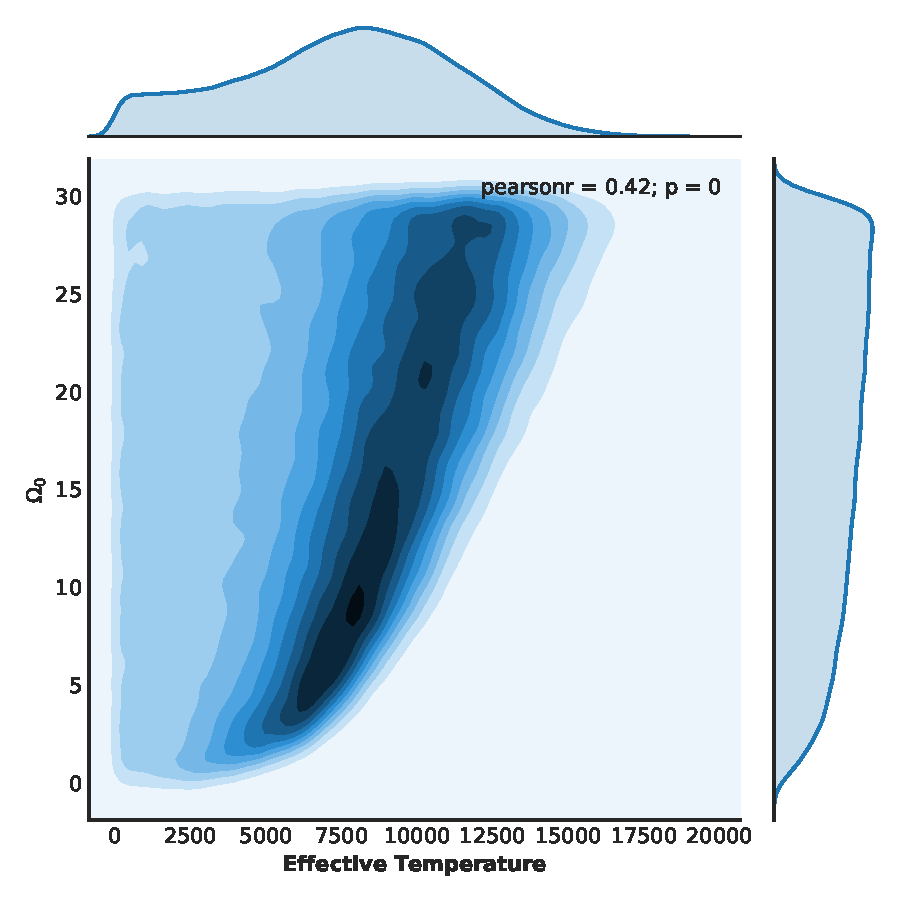
\includegraphics[width=0.42\linewidth]{prob2_kde.pdf}}\hfill%
    \subcaptionbox{\label{fig:mcmc_spectrum}}{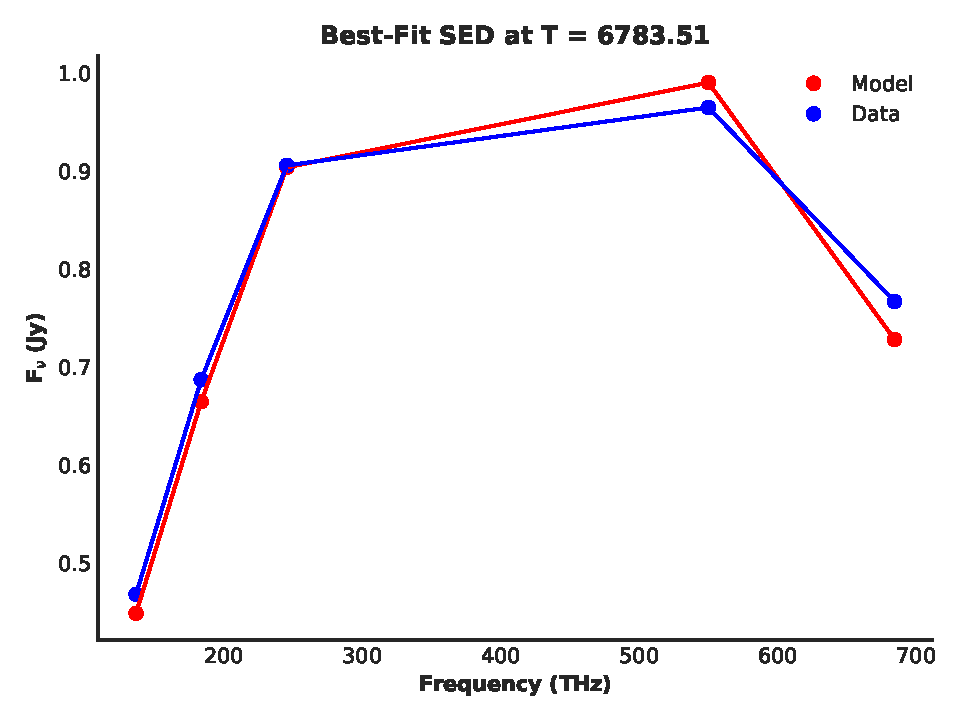
\includegraphics[width=0.52\linewidth]{prob2_spectrum.pdf}}\hfill%
    \hspace*{\fill}%
    \caption{Results from an MCMC fitting run. The kernel-density estimate (KDE) on the left characterizes the probability distribution of points in $\Omega_0-T$ parameter space, where darker regions correspond to better fits. On the right, data and best-fit model are overlaid, demonstrating that a good solution was found.}
  \end{figure}


  To run my MCMC, I developed a probability function that sampled a blackbody curve of a given temperature at the frequencies of the given data, then calculated a $\chi^2$ value between the data and model ($\chi^2 = \sum_i (\text{data} - \text{model})^2$), which was then turned into a log-probability ($\ln \text{prob} = -0.5 \chi^2$) value and fed back into the MCMC run, informing the run's next step. The log-probabilities are shown in Fig \ref{fig:mcmc_kde} in $\Omega_0-T$ parameter space.

  As we see, there is some degree of degeneracy between the two parameters. This is somewhat reasonable, since increases in temperature and solid angle-subtended will both result in increased flux density for a source. However, the resulting fit (Fig \ref{fig:mcmc_spectrum}) looks pretty splendid, returning a best-fit temperature of 6783K\footnote{This is a little bit strange. Obviously, this temperature results in a great fit, as shown by the spectrum, but it visually looks like the darkest part of the KDE, at least to my eye, is centered more towards 7500K or so. Still, the process of retrieving the best-fit values is an automated one (not something I do by hand), so I think this is more a problem with the KDE plot than with the fitting itself.}, which is characteristic of an F3 star. This is quite close to the F2 stellar type that is predicted by the star's 0.37 B-V color, indicating that the star is either truly an F3 that has been a bit reddened, or it is an F2 star that is slightly too cool.
\end{answer}




\bigskip \bigskip
\begin{problem}{3}
  Given the information on a fictitious star, as listed in the table below, determine its other properties. Present your results as a table and explain each calculation in comments below the table. \bigskip

  \centerline{Table of data on a fictious star}
  \smallskip
  \centerline{
  \begin{tabular} {cc}
  \hline \hline
  $\alpha,\delta$ & 13:42:25.6, -7:13:42.1 (J2000.00) \\
  $\mu$ & 13.7 mas y$^{-1}$ \\
  PA & 122\textdegree \\
  v$_r$ & -13 km s$^{-1}$ \\
  V & 10.86 \\
  B-V & 1.63 \\
  SpT & K2V \\
  \hline
  \end{tabular}
  }

  \bigskip

  \noindent {\bf Properties for you to determine and tabulate:} (l,b), M$_V$,  E(B-V), A$_V$, d, the magnitude of heliocentric space velocity (v$_{space})$, M$_{bol}$, L/L$_\odot$, T$_e$, R/R$_\odot$, and M/M$_\odot$. Explain how you obtained each of the requested quantities in comments below the table. In addition, comment on the likely age and chemical composition of this star and whether it is likely to have a planetary system. As always, justify your answers.
\end{problem}

\begin{answer}{3}

  \centerline{\textbf{Results}}
  \smallskip
  \centerline{
  \begin{tabular} {cc}
  \hline \hline
  l, b          & (324.52$^o$, 53.49$^o$) \\
  M$_V$         & 6.19 \\
  E(B-V)        & 0.75 \\
  A$_V$         & 2.25 \\
  d             & 30.48 pc \\
  v$_{space}$   & 2628 km s$^{-1}$ \\
  M$_{bol}$     & 5.9 \\
  T$_e$         & 5040 \\
  L/L$_\odot$   & 0.27 \\
  M/M$_\odot$   & 0.72 \\
  R/R$_\odot$   & 0.68 \\
  \hline
  \end{tabular}
  }

  \bigskip
  \textbf{How I found these values:}
  Many of these questions required looking up values in a table. For any question where this was the case (i.e. where I say "I looked up this value"), the table I am referring to can be found here: \url{http://www.pas.rochester.edu/~emamajek/EEM_dwarf_UBVIJHK_colors_Teff.txt}
  \begin{\begin{itemize}

    \item \textbf{l, b}: Using the calculator I made for the last problem set, I found that the (l, b) coordinates of this source are (324.52$^o$, 53.49$^o$).

    \item \textbf{E(B-V)}: Recalling the definition E(B-V) = (B-V) - (B-V)$_0$, where the first term is the observed color and the second term is the color we would expect from a star of this spectral type, we just have to look up this expected color and subtract it from the given B-V color. I looked up a value of (B-V)$_0$ = 0.884 for a K2V star which yields a value of E(B-V) = 0.75.

    \item \textbf{A$_V$ }: Recalling the definition A$_V$ = 3.1 E(B-V), we may just multiply our existing answer by 3.1. Doing so, we find A$_V$ = 2.25.

    \item \textbf{M$_V$}: Looking up in our table, we find that for a K2V star, M$_V$ = 6.19.

    \item \textbf{M$_{bol}$}: We recall that M$_{\text{bol}} = M_V + BC_V$, where $BC_V$ is the Bolometric Correction in the V-band, and can be looked up to be -0.29. This yields a result of M$_{bol}$ = M$_V$ + BC$_V$ = 6.19 - 0.29 = 5.9.

    \item \textbf{d}: We may rearrange the magnitude equation for distance:
    \begin{align*}
      V - M_V &= 5 \log{d} - 5 + A_V\\
      \rightarrow \log{d} &= \frac{V - M_V - A_V + 5}{5} = 1.48 \\
      \rightarrow d &= 10^{1.48} \\
                    &= 30.48 \text{ pc}
    \end{align*}

    \item \textbf{v$_{space}$}: The space velocity is the triangulation of the proper motion, $\mu$, and the radial velocity, i.e. $v_{space} &= \sqrt{ v_{rad}^2 + v_{trans}^2 }$. To solve this, we must turn proper motion into a velocity, using the familiar equation, $v_{trans} = 4.74\ \mu\ d = 4.74\ (13.7) (30.48) = 2628$ km s$^{-1}$}. Therefore, $v_{space} &= \sqrt{ (13)^2 + (2628)^2 } \approx 2628$ km s$^{-1}$}. This feels way too high, but I don't really have any justification to back up that intuition and the math seems tight, so I guess that's what I'll submit.

    \item \textbf{T$_{eff}$}: Looking it up, we find that for a K2V star, T$_{eff}$ = 5040.
    \item \textbf{L/L$_\odot$}: Since luminosity and magnitudes are related as $M - M_{\odot} = -2.5 \log{\frac{L}{L_{\odot}}}$, then we may look up values for $M$ and $M_{\odot}$ and find $\frac{L}{L_{\odot}} = 10^{-0.4\ (M - M_{\odot})} = 10^{-0.4\ (6.19 - 4.79)} = 0.27$
    \item \textbf{M/M$_\odot$}: From the Mass/Luminosity relation, we know that $\frac{M}{M_{\odot}} = \frac{L}{L_{\odot}}^{1/4} = 0.72$
    \item \textbf{R/R$_\odot$}: We may find the radius by first recalling:

    \begin{align*}
      T_{eff}^4 &= \frac{L}{4 \pi\ R^2 \sigma}
    \end{align*}

    Since we know T$_{eff}$ for our fictional star and the Sun (another lookup reveals that a G2V's effective temperature is 5770), and we know the two's luminosity ratio, we may construct the following ratio by rearranging the above equation and solving for the radius relationship:
    \begin{align*}
      \frac{L}{L_\odot} &= \frac{4 \pi\ R^2 T_{eff}^4}{4 \pi\ R_{\odot}^2 T_{eff, \odot}^4} \\
      \rightarrow \frac{R}{R_{\odot}} &= \sqrt{\frac{L}{L_\odot} \left(\frac{T_{eff, \odot}}{T_{eff}}\right)^4} \\
        &= \sqrt{0.27 \times \left(\frac{5770}{5040}\right)^4} \\
        &= 0.68
    \end{align*}

  Thus, $R/R_{\odot} \approx 0.55$.

  \end{itemize}}
\end{answer}


Given that this is a K-star, we expect it to have a high metallicity. Lower mass stars tend to live much longer, so it is more likely that this star is an older star than it's higher-mass companions.

To determine the star's planet forming potential, I decided to see what the real data say about planets around this type of star. To do so, I used the Python package \texttt{kplr}, an API wrapper of the Kepler database's data portal, to download information about $\sim$2300 planets. Each planet's information contained a field with information about it's host star. This allowed me to develop my own little database with features like metallicity, effective temperature, colors, and so on for each confirmed planet's host.

Unfortunately, one feature that my database did not yet contain was spectral type. This is obviously critical, since the whole point of this little project was to determine the relative frequency of planets around stars by spectral type. I decided to use effective temperature as a spectral type proxy, since it goes linearly with spectral type and I had access to good data on the spectral class/T$_{eff}$ relationship. To do this, I copied, processed, and tabulated the table that I used above for other reference values into a robust dataframe in Python. I was then able to iterate through each star in my database, cross-check its reported T$_{eff}$ against the list of effective temperatures in the linked table, and label the star with the spectral type attached to the nearest T$_{eff}$ value in the linked table. This is a somewhat sketchy way of spectral-typing stars and, were this a more serious project, is definitely something I would give more thought to, but for the time being, it gave me a good, quick way to get approximate spectral types.

\begin{figure}[htp]
  \hspace*{\fill}%
  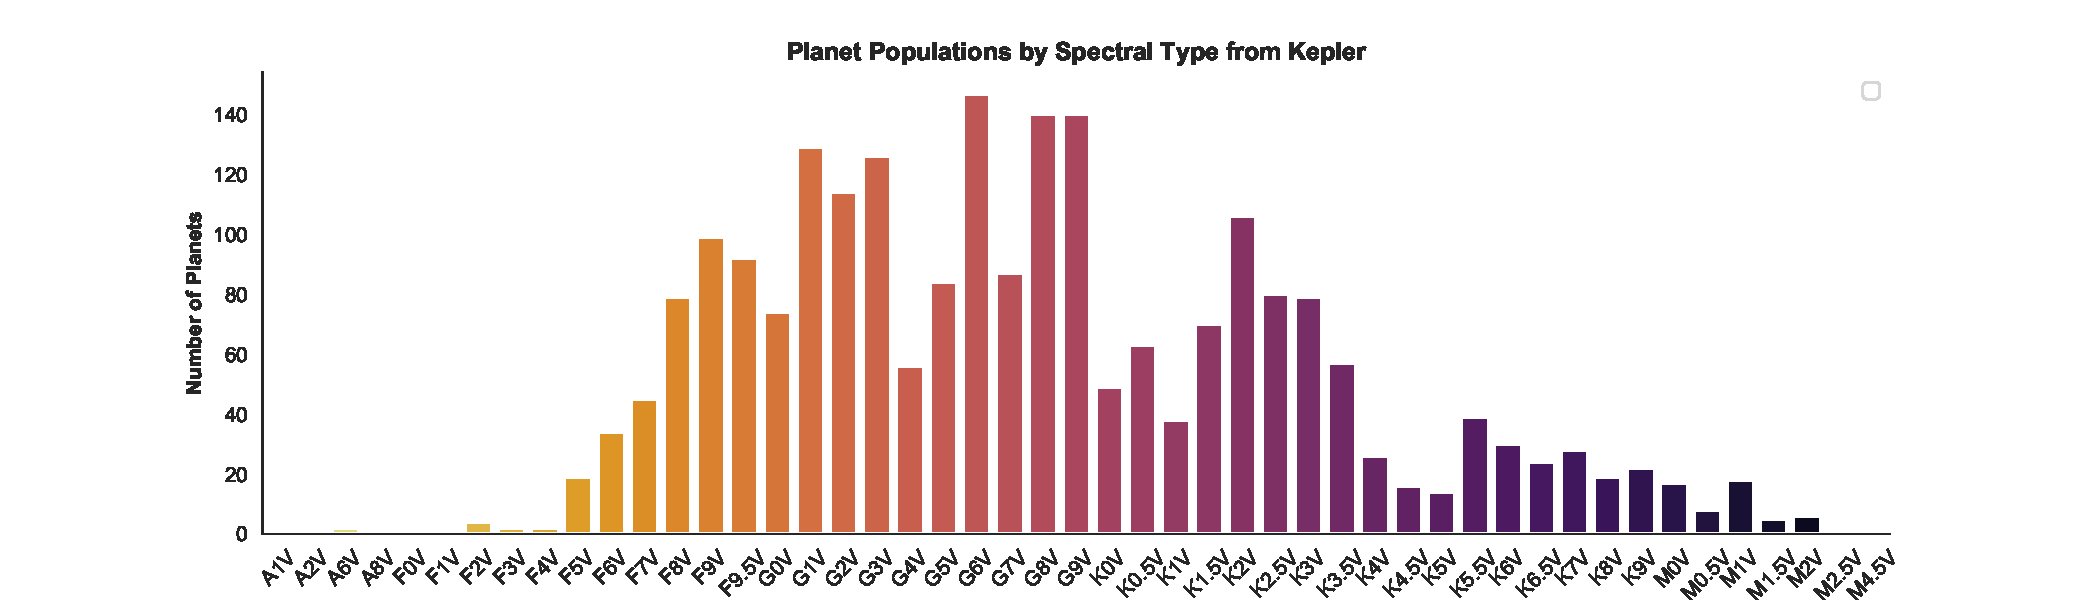
\includegraphics[width=\linewidth]{planet_dist_by_spt.pdf}\hfill%
  \hspace*{\fill}%
  \caption{Planetary populations around stars of different spectral types, drawn from Kepler data. Unfortunately, it's hard to set photos in a two-column layout, so the inclusion of this plot forced me back into a one-column submission. Still, I'm really excited about how the plot turned out, so I think it's worth it.}
  \label{fig:planet_pops}
\end{figure}


Once I had these types, it was simply a matter of making an histogram of the results.


\bigskip
\centerline{\textbf{Planet Counts by Spectral Class}}
\smallskip
\centerline{
  \begin{tabular} {ccccc}
  \hline \hline
  A  & F   & G    & K   & M \\
  5  & 378 & 1097 & 760 & 56 \\
  \hline
  \end{tabular}
  \label{table:spectral_group}
}
\bigskip
\bigskip

We can see from Table \ref{table:spectral_group} that K stars have the second most detections of planets orbiting them, trailing only our beloved G stars. This indicates that planet-forming potential is likely high. Zooming in on this particular star's subtype, a K2V star, we see from Fig \ref{fig:planet_pops} that this specific class actually has the highest planetary detection rate of all K-stars, and the seventh highest rate overall. Therefore, from this data, I would say its planet-forming potential is high.

\textsc{Note}: I have entirely ignored, of course, the very significant issue of detection bias in this dataset. For example, we know that planets are extremely common around M-dwarfs, but since they are faint and hard to detect, they are underrepresented in this distribution. Still, since this is nothing more than a first-order diagnostic and the fictious star in question happens to be of a spectral type that has lots of observed planets, I think it's a reasonable sacrifice to make. Also, while it might not be enormously informative of the "true" planet-forming potential, it certainly is a useful way to predict how likely it is that we'd actually be able to find a planet around it. Finally, my data is all from the Kepler mission; a more robust implementation would, at the very least, also draw on K2 data and hopefully would reach out to other telescopes as well.



\bigskip \bigskip
\begin{problem}{4}  Fun with magnitudes and colors! If a star with a parallax of 25 mas that initially appears to be single and is measured to have V=6.50, later turns out to be a spectroscopic binary with equal mass components, what is the apparent magnitude of each component? Neglecting reddening, what is the absolute magnitude of each component? If that same star has a measured B-V = 1.25, what is the B-V of each component?
\end{problem}


\begin{answer}{4}

Since magnitude is given by
\begin{align*}
  V &= -2.5 \log{\frac{f}{f_0}},
\end{align*}

then $f$, the flux of a star, is
\begin{align*}
  f/f_0 &= 10^{-0.4\ V}
\end{align*}

Therefore, given that the V-magnitude of a binary is V=6.5, then we know that
\begin{align*}
  (f_1 + f_2)/f_0 &= 10^{-0.4\ V} \\
                  &= 0.0025
\end{align*}

Given that the two sources have the same mass, we may draw on the Mass-Luminosity relationship (and recall that flux is just distance-scaled luminosity) to infer that they have the same fluxes. Therefore,the flux of one of the sources is
\begin{align*}
  f_1/f_0 &= \frac{0.0025}{2}
\end{align*}

We can now plug this value back into our original equation for magnitude and find a single source's contribution.
\begin{align*}
  V &= -2.5 \log{\frac{f_1}{f_0}} \\
    &= -2.5 \log{(1.25 \times 10^{-3})} \\
    &= 7.26 \\
\end{align*}

We find a final apparent V magnitude of 7.26 for each star. To find the B-V color of each component, we can play the same game as above, just in the B-band. Again,
\begin{align*}
B &= -2.5 \log{\frac{f}{f_0}} \\
\rightarrow f/f_0 &= 10^{-0.4\ B}.
\end{align*}
Since our apparent B-magnitude is B = 1.25 + (V = 6.5) = 7.75, then:
\begin{align*}
(f_1 + f_2)/f_0 &= 10^{-0.4\ B} \\
                &= 7.94 \times 10^{-4}
\end{align*}

Again, we may recall that the two sources have the same mass and thus the same flux contributions, so
\begin{align*}
f_1/f_0 &= \frac{0.000794}{2}
\end{align*}

We can now plug this value back into our original equation for magnitude and find a single source's contribution.
\begin{align*}
B &= -2.5 \log{\frac{f_1}{f_0}} \\
  &= -2.5 \log{(3.97 \times 10^{-4})} \\
  &= 8.51 \\
\end{align*}

We see that each source has an apparent B-magnitude of 8.51, resulting in B-V color of 8.51-7.26 = 1.25, the same as the binary's combined color. I guess this is fairly obvious; the combined color of two identical sources should be the same as the color of each source. Still, it's pretty neat to get to walk through the actual equations themselves and see that that relationship does, in fact, hold.

To find the star's absolute magnitude, we recall the relationship between apparent magnitude, absolute magnitude, and distance.
\begin{align*}
  V - M &= 5 \log{d} - 5 + A_V
\end{align*}

Here $d = \frac{1}{25 \text{ mas}} = 400$ pc and $A_V$, the reddening, is taken to be zero. Therefore,
\begin{align*}
  M &= V - 5 \log{400} + 5 + 0 \\
    &= -0.75,
\end{align*}

so each star has an absolute magnitude in the V-band of -0.75. This is quite bright, perhaps a bit brighter than what I'd expect, but I guess it is quite far away, so maybe that does make sense.








\end{answer}







\begin{problem}{5}
More fun with magnitudes and colors! Suppose a binary system is composed of an A star, with V = 7.80 and B-V = 0.00, and a K star, with V = 8.20 and B-V = +1.50. If the stars are so close together on the sky that that they cannot be resolved as individual objects (i.e. an unresolved binary), what will be the measured V magnitude and B-V color of the ``star" (that is actually the combined light of both components)?
\end{problem}

\begin{answer}{5}
  We may use the same logic as before again to find the star's fluxes in each band and then work backward to single-source magnitudes.

  \begin{align*}
    f_{A, V}/f_0 &= 10^{-0.4\ V_{A, V}} \\
                 &= 7.59 \times 10^{-4} \\
    f_{A, B}/f_0 &= 10^{-0.4\ V_{A, B}} \\
                 &= 7.59 \times 10^{-4} \\
    f_{B, V}/f_0 &= 10^{-0.4\ V_{B, V}} \\
                &= 5.25 \times 10^{-4} \\
    f_{B, B}/f_0 &= 10^{-0.4\ V_{B, B}} \\
                &= 1.32 \times 10^{-4} \\
  \end{align*}

  Combining sources A and B's V-band and B-band fluxes, we find:
  \begin{align*}
    V_{both} &= -2.5 \log{[(7.59 + 5.25) \times 10^{-4}]} \\
               &= 7.23 \\
    B_{both} &= -2.5 \log{[(7.59 + 1.32) \times 10^{-4}]} \\
              &= 7.96 \\
  \end{align*}

Solving, we find that the binary would present as a star with V=7.23, B-V=0.73.


\end{answer}





%\end{multicols*}
\vfill\eject
\clearpage


\lstinputlisting[language=Python]{scratch_hw2.py}
\lstinputlisting[language=Python]{spt_data.py}

% How to include a PDF:
%\includegraphics [scale=0.4] {SamplePDF.pdf}




\end{document}
